\documentclass[10pt, uplatex, dvipdfmx]{jsarticle}
\usepackage{../mypackage}

\graphicspath{{../pictures}}

\setcounter{section}{11}

\begin{document}


\section{体積と面積と曲面積}

 \subsection{2重積分と体積}
 
 \begin{theorem}\label{thm:volume}
  $f,g$ を有界閉領域 $D \subset \mathbb{R}^2$ 上重積分可能な関数と
  し,$D$ 上で $f(x,y) \geqq g(x,y)$ とする.$D$ から $xy$ 平面に垂直に
  生やした柱と曲面 $z=f(x,y)$ と $z=g(x,y)$
  で囲まれた立体
  \[
    V=\Set{ (x,y,z) | (x,y) \in D, \, g(x,y) \leqq z \leqq
      f(x,y)}
  \]
  の体積は2重積分 $\ds \iint_{D} \Big( f(x,y) - g(x,y) \Big) dx dy$ に等しい.
  \begin{figure}[h]
    \centering
    \includegraphics[height=6cm]{07/monotonic.png}
  \end{figure}
\end{theorem}

\begin{example}\label{ex:volsphere}
  半径 $R>0$ の球の体積 $V(R)$ は $D=\Set{(x,y) | x^2+y^2 \leqq R^2}$ 上
  の以下の2重積分で求められる.
  \begin{align*}
    V(R) &= \iint_{D} \left( \sqrt{R^2-x^2-y^2} - \left(-\sqrt{R^2-x^2-y^2}\right)\right) dx dy\\
         & = 2\iint_{E} r\sqrt{R^2-r^2}\  dr d\theta 
           \quad \Big( E=\Set{(r, \theta) | 0 \leq r \leq R, \, 0 \leq \theta \leq 2\pi}\Big)\\
         & = 2 \int_{0}^{2\pi} \left( \int_{0}^{R} r \sqrt{R^2-r^2} \ dr \right) d\theta
           = 4\pi \left[ -\frac{1}{3} \left(R^2-r^2\right)^{\frac{3}{2}}\right]_{r=0}^{r=R}
           =\frac{4}{3}\pi R^3
  \end{align*}
  \begin{figure}[h]
    \centering
    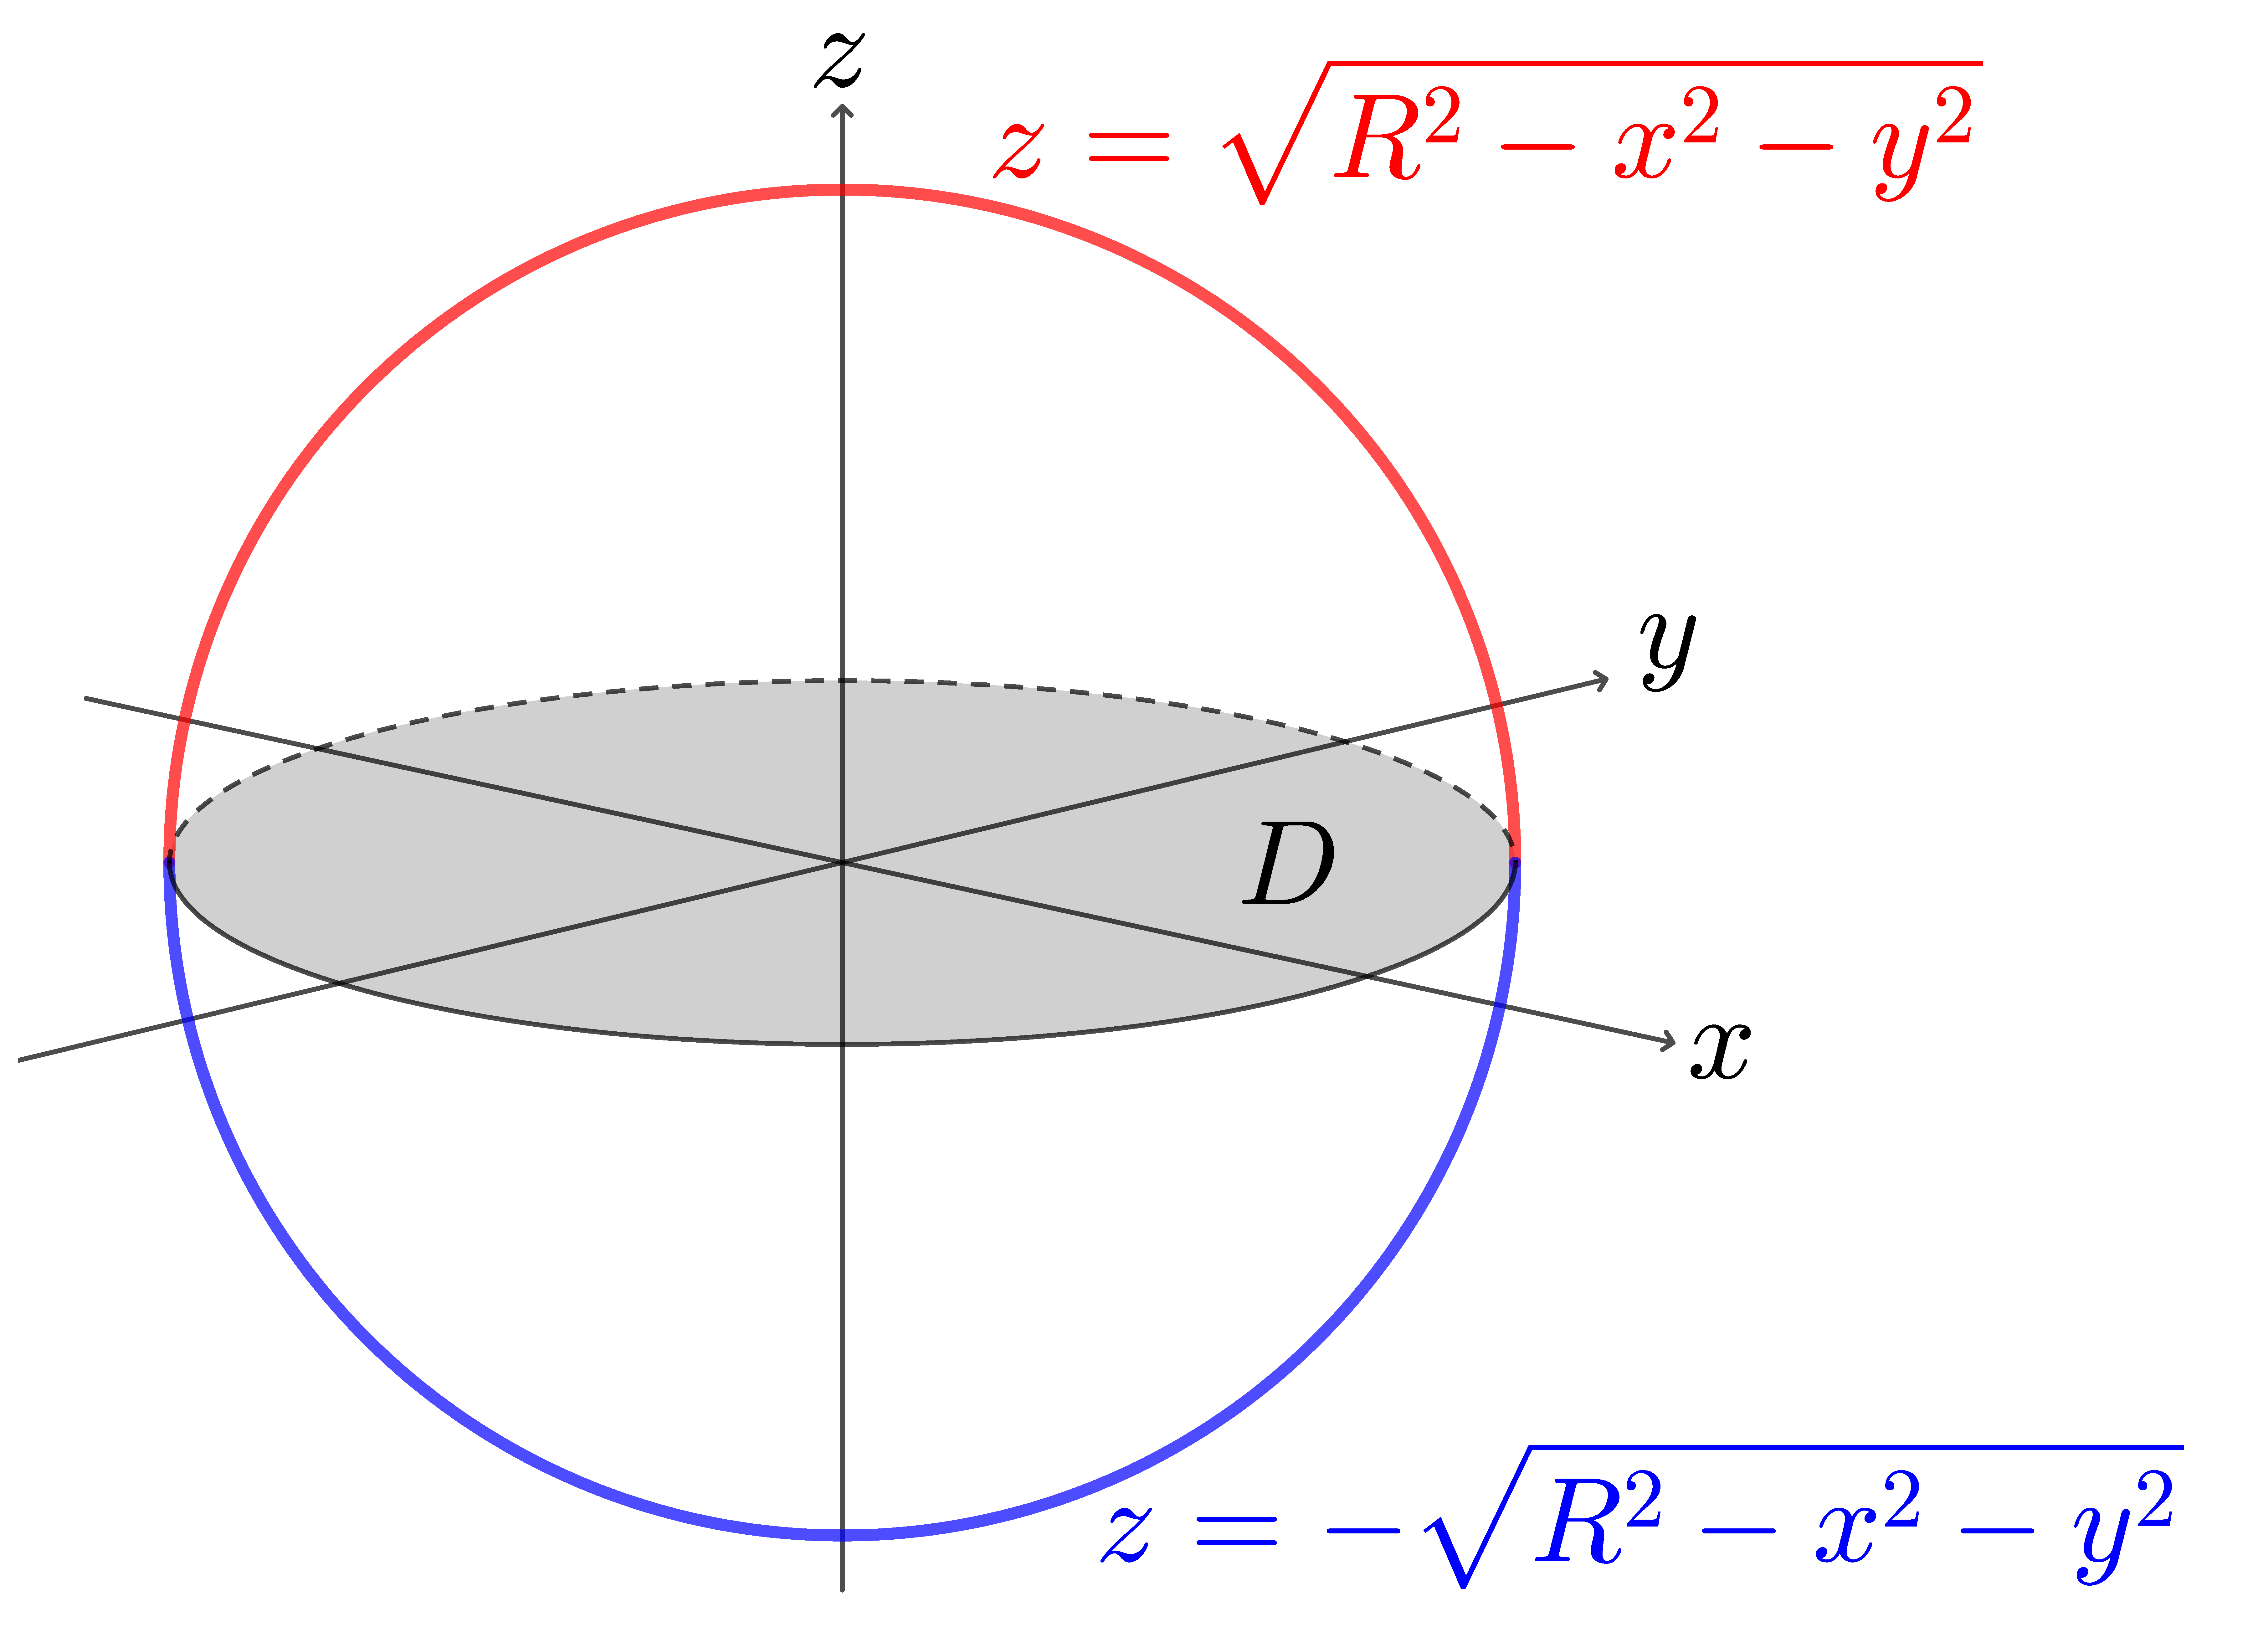
\includegraphics[height=5cm]{12/sphere2d.pdf}
  \end{figure}
\end{example}

\begin{example}
  下図のような曲面 $z=x^2+y^2$ と平面 $z=2x$ で囲まれる立体の体積を求める.
  \begin{figure}[h]
    \centering
    \includegraphics[width=10cm]{12/cutparab.png}
  \end{figure}

  平面 $z=2x$ が曲面 $z=x^2+y^2$ より上部にある閉
  領域上で2重積分を計算すればよい.つまり,
  \[
    D= \Set{(x,y) \ \mid x^2+y^2 \leqq 2x}
  \]
  として,2重積分 $\ds \iint_{D} \left( 2x - \left(x^2+y^2\right) \right) \ dx dy$ を計算する.\\

  簡単な不等式の変形により,$D$ は点 $(1,0)$ を中心とする半径 $1$ の円板であるこ
  とがわかる.そこで,極座標変換と $x$ 方向の平行移動を合成した変
  換
  \[
    \begin{cases}
      x = r\cos \theta+1\\
      y = r\sin \theta
    \end{cases}
  \]
  を使う.この変換によって $r\theta$ の閉領域
  \[
    E = \Set{(r, \theta) \ \mid \ 0 \leqq r \leqq 1, \; 0 \leqq \theta \leqq 2\pi}
  \]
  が $D$ に変換される.変換の Jacobian は
  \[
    J(r,\theta) = \left|
      \begin{array}{cc}
        \frac{\partial x}{\partial r} & \frac{\partial x}{\partial \theta}\\[1ex]
        \frac{\partial y}{\partial r} & \frac{\partial y}{\partial \theta}
      \end{array}
    \right| = \left|
      \begin{array}{rr}
        \cos \theta & -r\sin\theta\\[1ex]
        \sin \theta & r\cos\theta
      \end{array}
    \right| = r
  \]
  なので,求めたい体積は次のように計算できる.
  \[
    \iint_{D} \left( 2x- \left(x^2+y^2\right) \right) \ dx dy
    = \iint_{E} \left(1-r^2\right) r \ dr d\theta 
    = \int_{0}^{2\pi}\left( \int_{0}^{1} \left(r-r^3\right)dr \right) d\theta = \frac{\pi}{2}
  \]
\end{example}

\newpage

\subsection{2重積分と面積}

$xy$ 平面内の有界閉領域 $D$ を底面とする高さ $1$ の立体の体積は $D$ の
面積に等しい.

\begin{theorem}\label{thm:doublearea}
  定数関数が重積分可能な有界閉領域 $D$ の面積は2重積分 $\ds \iint_{D}dxdy$ の値に等しい.
  \begin{figure}[h]
    \centering
    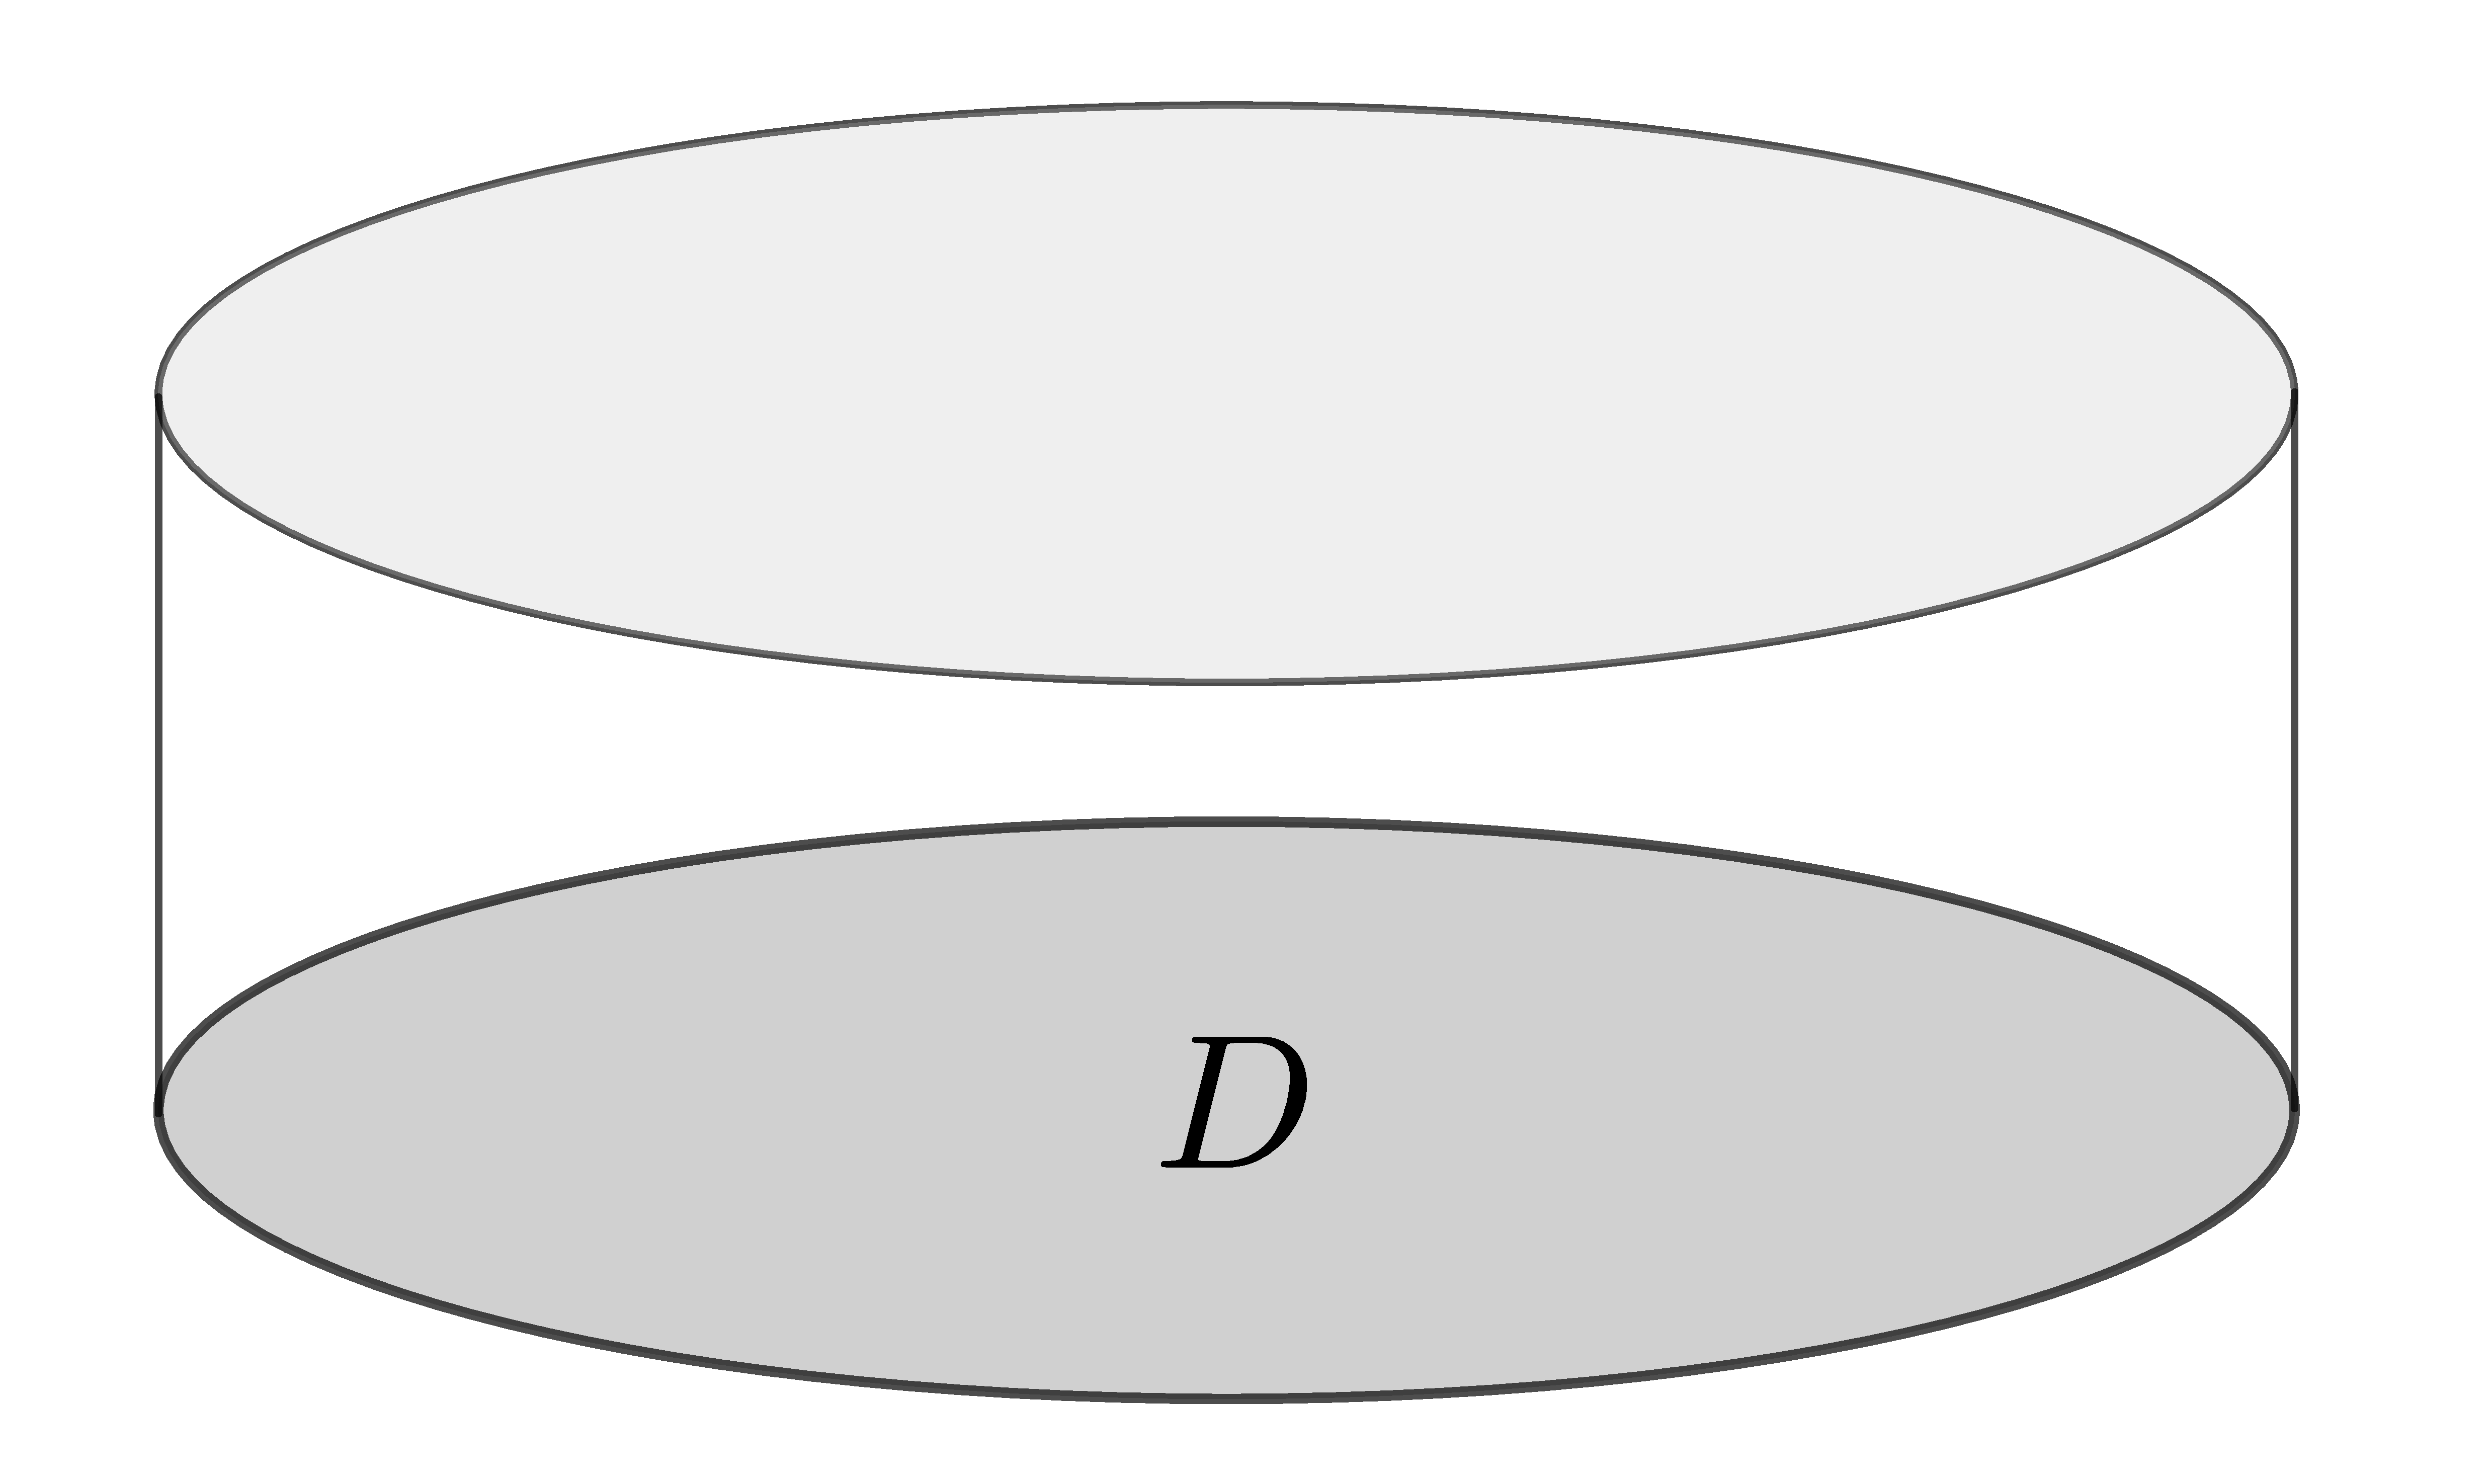
\includegraphics[width=10cm]{12/volume-area.pdf}
  \end{figure}
\end{theorem}

\begin{example}
  半径 $R>0$ の円の面積 $S(R)$ は $1$ 変数関数の積分で求められるが,定
  理\ref{thm:doublearea}より
  \[
    D=\Set{(x,y) | x^2+y^2 \leqq R}
  \]
  上で定数関数の$2$ 重積分を計算しても求められる.
  \[
    S(R) = \iint_{D} dx dy = \int_{-R}^{R} \left(\int_{-\sqrt{R^2-x^2}}^{\sqrt{R^2-x^2}} dy \right) dx
    = \int_{-R}^{R} \left( \sqrt{R^2-x^2} - \left(-\sqrt{R^2-x^2} \right) \right) \ dx = \pi R^2
  \]
\end{example}

\vspace{1zh}

この例を見てわかるように,定理\ref{thm:doublearea}を使ったからといって
特に計算が楽になる訳でもなく,途中からこれまで通りの1変数の積分計算に合
流している.より一般に,有界閉領域 $D$ が縦線集合として
\[
  D=\Set{(x,y) \ \mid \ a \leqq x \leqq b, \; \varphi_1(x) \leqq y \leqq \varphi_2(x)}
\]
と書けるなら $D$ 上の定数関数 $z=1$ の2重積分は次のように計算される.
\[
  \iint_{D} dx dy = \int_{a}^{b} \left( \int_{\varphi_1(x)}^{\varphi_2(x)} \ dy \right) dx
  = \int_{b}^{a} \Big( \varphi_2(x) - \varphi_1(x) \Big) \ dx
\]
これは結局 $y=\varphi_1(x)$ と $y=\varphi_2(x)$ と $x=a$ と $x=b$ で囲
まれる平面図形 $D$ の面積を求める積分である.$D$ が横線集合として書ける
ときも全く同様である.\\

「だから定理\ref{thm:doublearea}なんて意味がない」と主張したい
訳\textbf{ではない}.むしろこの定理によって定数関数の2重積分に面積という意味
付けが与えられる.

\newpage

\subsection{立体の断面積と積分と体積}

立体の断面積を積分すればその立体の体積が得られる.

\begin{theorem}\label{thm:area-section}
  $xyz$ 空間にある立体を $x$ 軸に垂直な平面 $x=\xi$ で切断したときの断
  面積が $S(\xi)$ であり,この立体が $a\leqq x \leqq b$ の範囲に含
  まれているとする.関数 $S(x)$ が有界閉区間 $[a,b]$ で積分可能な
  ら,この立体図形の体積は以下の積分値に等しい.
  \[
    \int_{a}^{b} S(x) \ dx
  \]
  \begin{figure}[h]
    \vspace{-1cm}
    \centering
    \includegraphics[height=5cm]{12/section.pdf}
  \end{figure}
\end{theorem}


\begin{remark}
  当たり前だが,$x$ 軸だけに限らず $y$ 軸や $z$ 軸についてもこの定理と
  同様のことが成り立つ.さらには,座標軸だけに限らず空間の任意の直
  線とそれに垂直な平面での断面積に関して同様のことが成り立つ.
\end{remark}

\begin{example}
  放物線 $y=x^2$ を $x$ 軸の周りで回転させて得られる回転体の $0 \leqq
  x \leqq 1$ の部分の体積を求める.
  
  \begin{figure}[h]
    \centering
    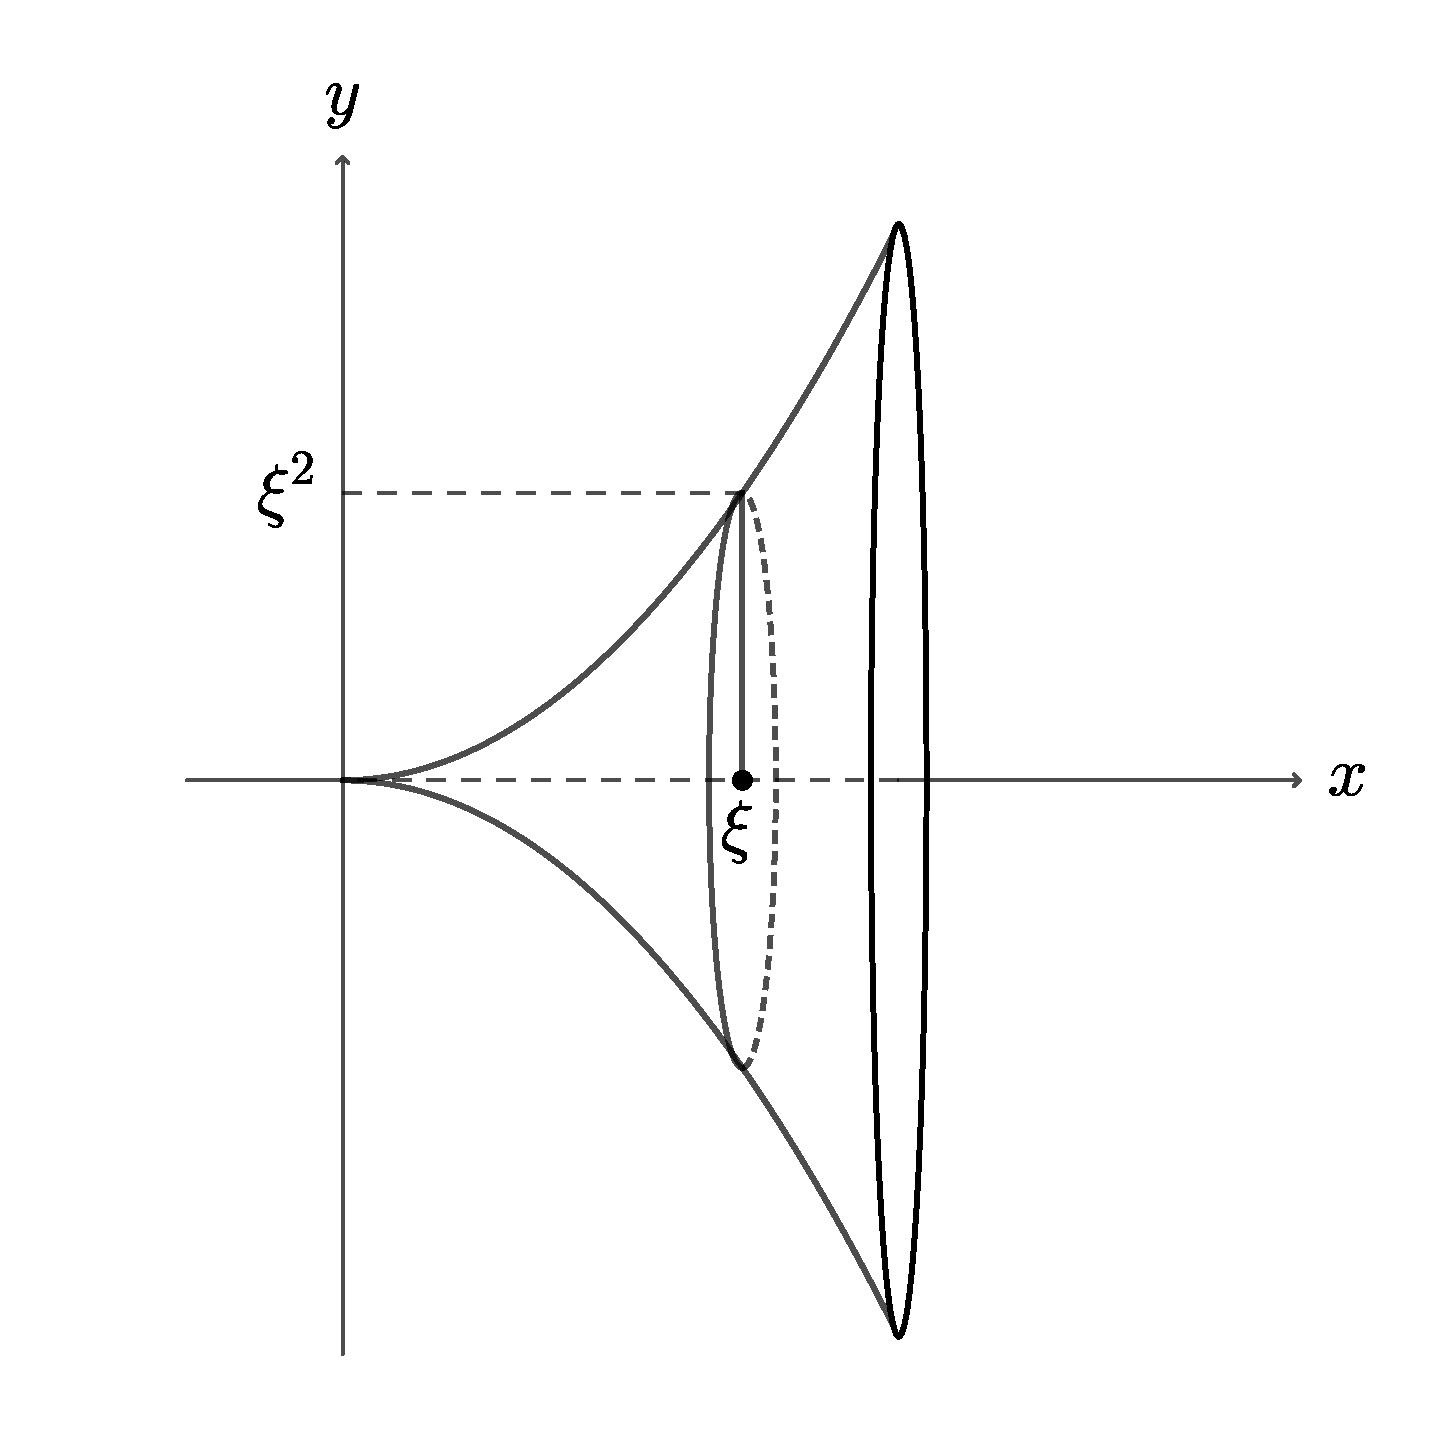
\includegraphics[height=7cm]{12/revolution.pdf}
  \end{figure}

  \noindent
  この立体を平面 $x=\xi$ で切断したと
  きの断面は半径 $\xi^2$ の円なので,その面積は $\pi \xi^4$ である.
  従って,定理\ref{thm:area-section}からこの立体の体積は以下のように計
  算できる.
  \[
    \int_{0}^{1} \pi x^4 \ dx = \pi \left[ \frac{x^5}{5}\right]_{0}^{1} = \frac{\pi}{5}
  \]

\end{example}
\newpage

\subsection{曲面積}


$\varphi, \psi, \chi$ を $uv$ 平面内の有界閉領域 $D$ 上定義され
た $C^1$ 級関数とする.点 $(u,v)$ が $D$ を動くとき,$xyz$ 空間内の
点 $\left( \varphi(u,v), \psi(u,v), \chi(u,v)\right)$ はなめらかな曲
面 $S$ を描く.これを
\[
  x=\varphi(u,v), \; y=\psi(u,v), \; z=\chi(u,v), \; (u,v) \in D
\]
と書き,曲面 $S$ の\textbf{媒介変数表示}という.

\begin{theorem}\label{thm:surface-area}
  有界閉領域 $D$ 上の $C^1$ 級関数 $\varphi, \psi, \chi$ によって媒介変
  数表示される曲面の面積は
  \[
    \iint_{D} \sqrt{\left( \frac{D(x,y)}{D(u,v)}\right)^2 + \left( \frac{D(y,z)}{D(u,v)}\right)^2 
      + \left( \frac{D(z,x)}{D(u,v)}\right)^2} \ du dv
  \]
  に等しい.ただし,ここで
  \[
    \frac{D(x,y)}{D(u,v)} = \left|
      \begin{array}{cc}
        x_u & x_v\\
        y_u & y_v
      \end{array}
    \right|, \quad \frac{D(y,z)}{D(u,v)} = \left|
      \begin{array}{cc}
        y_u & y_v\\
        z_u & z_v
      \end{array}
    \right|, \quad \frac{D(z,x)}{D(u,v)} = \left|
      \begin{array}{cc}
        z_u & z_v\\
        x_u & x_v
      \end{array}
    \right|
  \]
  であり,被積分関数は $D$ 上重積分可能であるとする.
\end{theorem}

\begin{example}
  半径 $R >0$ の球面は以下の媒介変数表示で与えられる.
  \[
    x = R\cos\theta  \cos \varphi, \quad
    y= R \sin \theta \cos\varphi, \quad
    z = R \sin \varphi, \quad 
    0\leqq \theta \leqq 2\pi, \; -\frac{\pi}{2} \leqq \varphi \leqq \frac{\pi}{2}
  \]
  \begin{figure}[h]
    \vspace{-2.5zh}
    \centering
    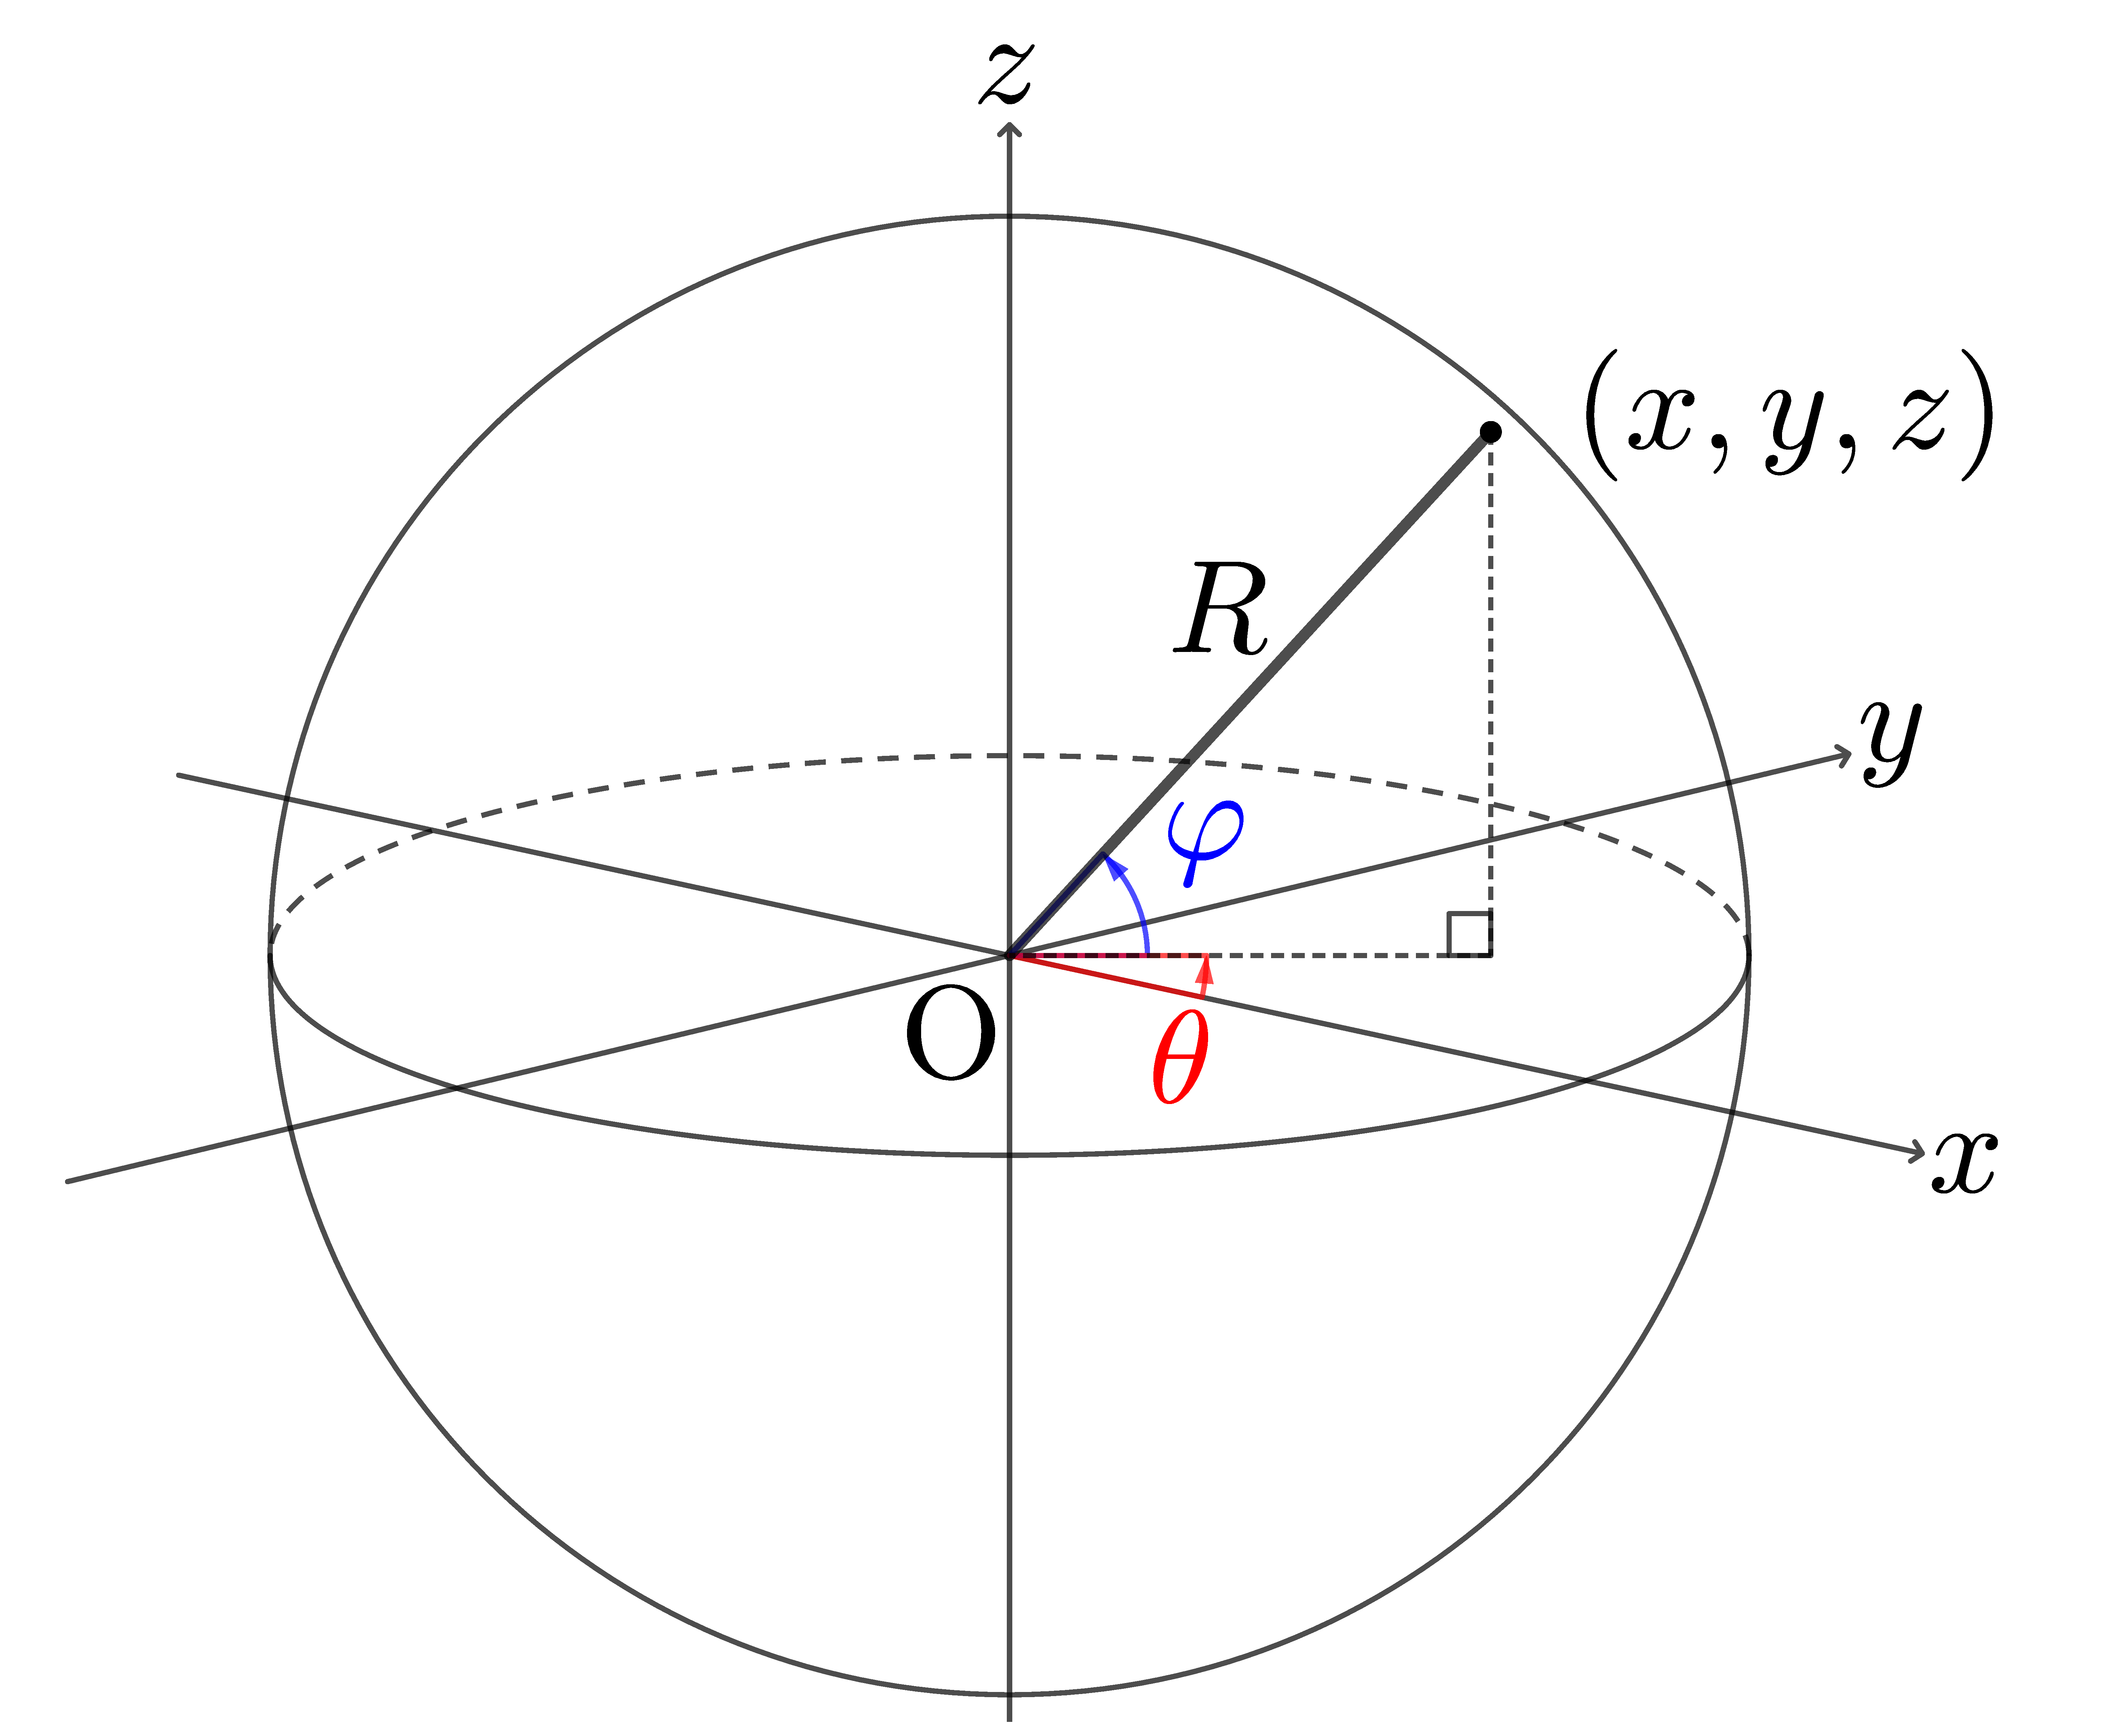
\includegraphics[height=4.7cm]{12/pole3d.pdf}
  \end{figure}

  曲面積の計算に必要な3個の Jacobian は以下の通りである.
  \[
    \begin{aligned}
    \frac{D(x,y)}{D(\theta, \varphi)} &= \left|
             \begin{array}{cc}
               x_{\theta} & x_{\varphi}\\
               y_{\theta} & y_{\varphi}
             \end{array}
           \right| = \left|
             \begin{array}{rr}
               -R \sin\theta \cos\varphi & -R \cos\theta \sin \varphi\\
               R \cos\theta \cos\varphi & -R \sin\theta \sin\varphi
             \end{array}
           \right| = R^2 \cos\varphi\sin\varphi\\[1ex]
      \frac{D(y,z)}{D(\theta, \varphi)} &= \left|
                                          \begin{array}{cc}
                                            y_{\theta} & y_{\varphi}\\
                                            z_{\theta} & z_{\varphi}
                                          \end{array}
                                          \right|= \left|
                                          \begin{array}{cc}
                                            R\cos\theta \cos\varphi & -R\sin\theta\sin\varphi\\
                                            0 & R\cos\varphi
                                          \end{array}
                                          \right| = R^2 \cos\theta \cos^2\varphi\\[1ex]
      \frac{D(z,x)}{D(\theta,\varphi)} &=\left|
                                        \begin{array}{cc}
                                          z_{\theta} & z_{\varphi}\\
                                          x_{\theta} & z_{\varphi}
                                        \end{array}
                                        \right| = \left|
                                         \begin{array}{cc}
                                           0 & R\cos\varphi\\
                                           -R\sin\theta\cos\varphi & -R\cos\theta\sin\varphi
                                         \end{array}
                                         \right| = R^2 \sin\theta \cos^2\varphi
    \end{aligned}
  \]
  これより半径 $R$ の球の表面積 $S(R)$ は
  $\ds D= \left[ 0, 2\pi \right] \times \left[ -\frac{\pi}{2},
    \frac{\pi}{2}\right]$ 上の2重積分として以下のように計算できる.
  \[
    \begin{aligned}
      S(R) &= \iint_{D} \sqrt{\left( \frac{D(x,y)}{D(\theta, \varphi)}\right)^2
             +\left( \frac{D(y,z)}{D(\theta,\varphi)}\right)^2 + \left( \frac{D(z,x)}{D(\theta,\varphi)}\right)^2
             } d\theta d\varphi
             = \iint_{D}R^2 \left|\cos \varphi\right| \ d\theta d\varphi\\
           &=R^2 \left( \int_{0}^{2\pi}d\theta\right)\left(\int_{-\frac{\pi}{2}}^{\frac{\pi}{2}}\cos\varphi\ d\varphi\right)
             = 4\pi R^2
    \end{aligned}
  \]
  
\end{example}

$C^1$ 級関数 $z=f(x,y)$ のグラフとして与えられる曲面は
\[
  x=u, \; y=v, \; z=f(u,v), \; (u,v) \in D
\]
と媒介変数表示できる.このとき
\[
  \frac{D(x,y)}{D(u,v)} = \left|
    \begin{array}{cc}
      1 & 0\\
      0 & 1
    \end{array}
    \right| = 1, \quad \frac{D(y,z)}{D(u,v)} = \left|
      \begin{array}{cc}
        0 & 1\\
        f_x & f_y
      \end{array}
    \right| = -f_x, \quad \frac{D(z,x)}{D(u,v)} = \left|
      \begin{array}{cc}
        f_x & f_y\\
        1 & 0
      \end{array}
    \right| = -f_y
\]
なので,定理\ref{thm:surface-area}の特別な場合として以下の定理が得られる.

\begin{theorem}\label{thm:function-area}
  有界閉領域 $D$ 上の $C^1$ 級関数 $z=f(x,y)$ のグラフの曲面積は以下の
  積分で与えられる.ただし,被積分関数は $D$ 上重積分可能であるとする.
  \[
    \iint_{D} \sqrt{ 1 + f_x(x,y)^2 + f_y(x,y)^2} \ dx dy
  \]
\end{theorem}

\begin{example}
  半径 $R>0$ の球の表面積 $S(R)$ は,2変数関数 $z=\sqrt{R^2-x^2-y^2}$の
  グラフの曲面積の $2$
  倍なので,$D=\Set{(x,y) | x^2+y^2 < R^2}$上の広義2重積分として以下の
  ようにも計算できる.
  \[
    S(R) = 2\iint_{D}\sqrt{ 1 + {z_x}^2 + {z_y}^2} \ dx dy 
    =  2R \iint_{D} \frac{dxdy}{\sqrt{R^2-x^2-y^2}} = 4\pi R^2
  \]
\end{example}

\begin{example}
  放物線をその軸の周りで回転して得られる回転放物面 $z=x^2+y^2$ の $x^2+y^2
  \leqq 1$ の部分の表面積を求める.つまり,$D=\Set{(x,y) \ \mid \
    x^2+y^2 \leqq 1}$ として,以下の2重積分を計算する.
  \[
    \iint_{D} \sqrt{1+z_x^2 + z_y^2} \ dx dy = \iint_{D} \sqrt{1+4x^2+4y^2} \ dx dy
  \]
  極座標変換 $x=r\cos\theta, y=r\sin\theta$ によって,$r\theta$ 平面の
  \[
    E = \Set{(r, \theta) \ \mid \ 0 \leqq r \leqq 1, \; 0 \leqq 0 \leqq 2\pi}
  \]
  が $xy$ 平面の $D$ に変換される.極座標変換の Jacobian は $J(r,\theta)=r$ なので,以下のように計算できる.
  \[
    \begin{aligned}
      \iint_{D} \sqrt{1+4x^2+4y^2} \ dx dy
      &= \iint_{E} \sqrt{1+4r^2} ~| J(r, \theta)| \ dr d\theta
        = \left(\int_{0}^{2\pi}\ d\theta\right) \left( \int_{0}^{1} r \sqrt{1+4r^2} \ dr \right)\\[1ex]
      &= 2\pi \left[ \frac{1}{12} \left( 1+4r^2\right)^{\frac{3}{2}}\right]_{0}^{1}
        = \frac{\pi\left(5\sqrt{5}-1\right)}{6}
    \end{aligned}
  \]
  \begin{figure}[h]
    \centering
    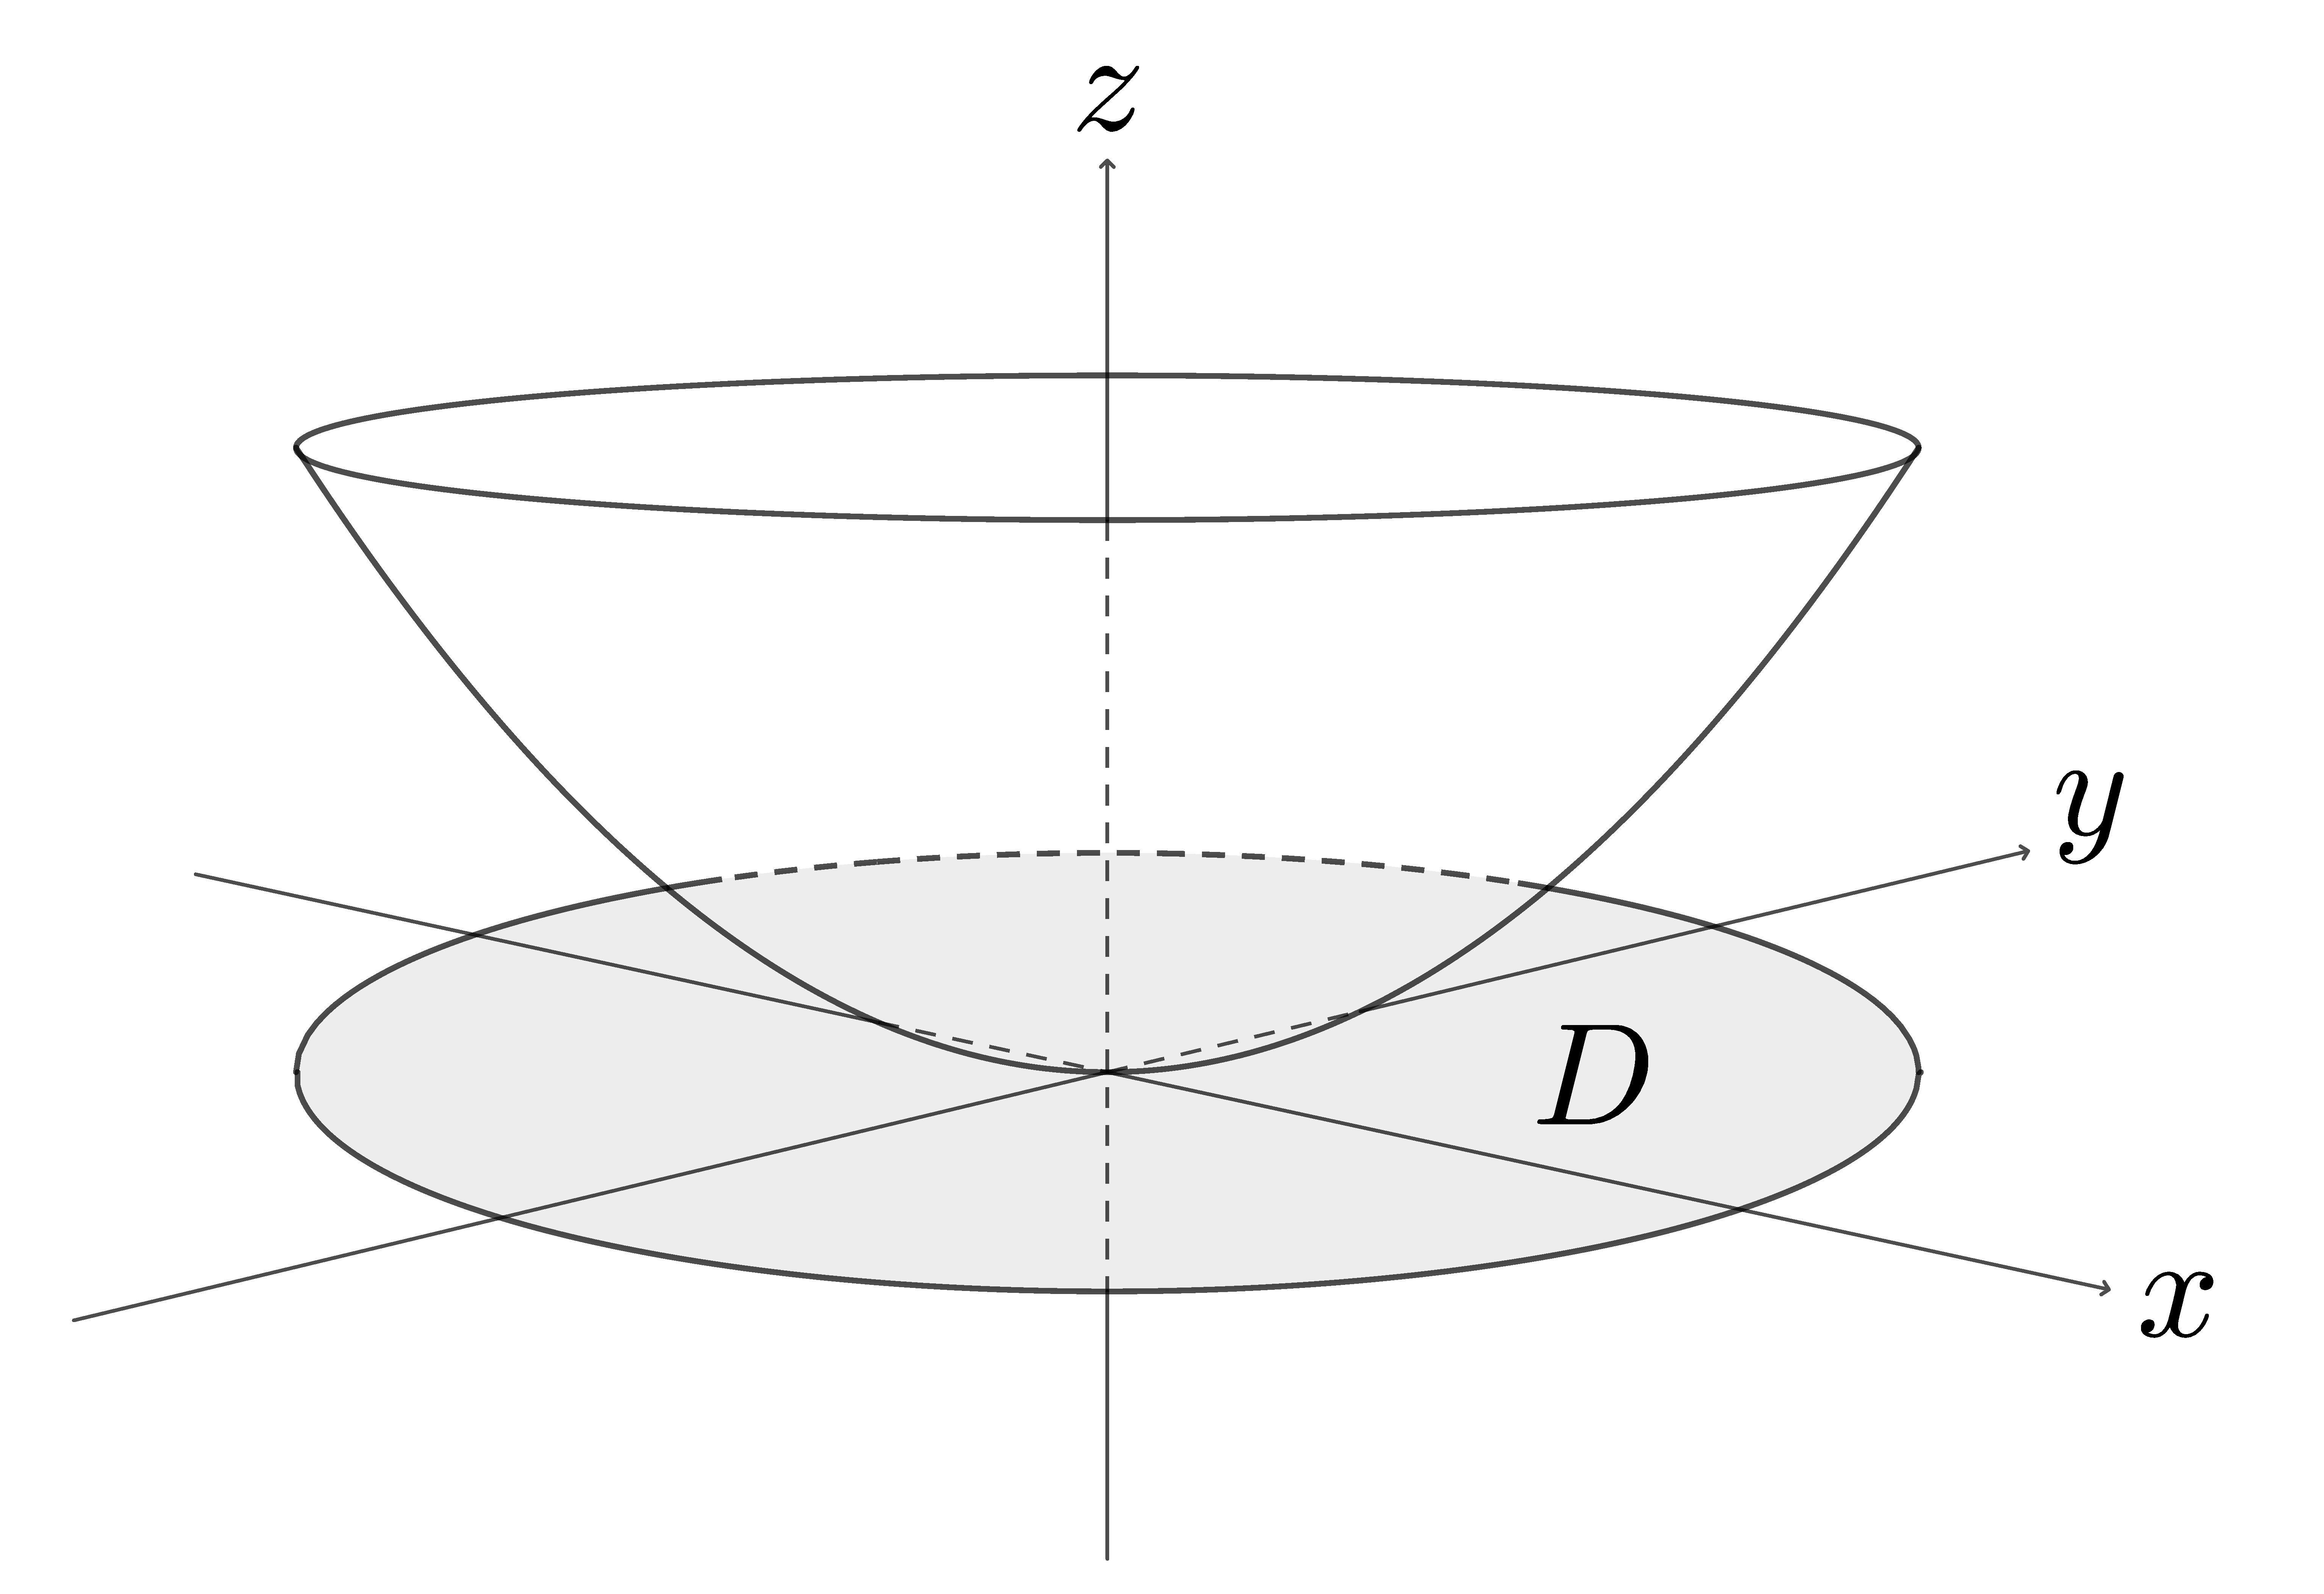
\includegraphics[height=4cm]{12/paraboloid.pdf}
  \end{figure}
\end{example}


\end{document}
